% literature review

\section{Introduction}

The previous chapter introduced the social network construct and explained how social network analysis can provide specific detail on knowledge sharing mechanisms and knowledge sharing behaviour. Deeper analysis involves applying relevant psychological or social theory to develop propositions or test hypotheses about specific social interactions. This chapter explores key psychological and social theories relevant to tacit knowledge sharing. \medskip

A key management challenge in open innovation for participants to willingly share their knowledge with other participants as needed, to align thinking and collaborative action. Participants cannot be coerced to share personal knowledge, especially tacit knowledge, which is a significant source of personal power. Sharing tacit knowledge is an act of volition or free-will. The structure versus agency debate provides a useful starting point to better understand the nature of volition, and what this means in terms of tacit knowledge sharing generally, and open innovation practice in particular. \medskip

Structure refers to the patterned arrangements that influence or limit the choices and opportunities available to individuals. Agency is the capacity of individuals to act independently and make their own free choices \citep{barker2016cultural}. Structure is about human efforts to organise, guide and regulate individual or group actions \citep{bandura1999social}. Though such structures shape human actions, human actions also shape or constitute social structures \citep{sewell1992theory}. The duality of structure refers to the extent an individual acts as a free agent or in a manner dictated by social structure \citep{giddens1984constitution}. \medskip

With open innovation, we need to consider how the structures of each partner organisation and the partnership itself, might influence knowledge sharing. For example, too much structure in an open innovation partnership may inhibit the sharing and co-creation of knowledge. Too little structure, on the other hand, may result in a lack of focus or chaos, leading to an unsatisfactory outcome. Proponents of open innovation might need to consider how structure may potentially impact knowledge sharing behaviour in open innovation partnerships. This may include developing skills to balance the need for formal structures with the individual need for autonomy. Past studies show innovation mostly happens through through informal structures \citep{allen1977role,ibarra1993network,selnes2003promoting}. The emergence of informal structures represents acts personal agency  Thus, managers need to consider how structure allow participants sufficient agency to develop their own informal relationships within a structured partnership.  

This includes allowing the emergence of informal structures that produce innovation. Understanding what motivates people to share and/or broker tacit knowledge is a good first step. Sharing tacit knowledge requires relatively high levels of motivation and trust. It is also about empowering others to perform work. \medskip 

This chapter considers theories of motivation, trust, and power and how these constructs might reflect structure, culture, and the influence of agency in open innovation partnerships. Brokerage can reveal much about motivation, trust, and power in knowledge networks. Patterns of brokerage can shed light on how people are motivated to share tacit knowledge. For example, are people motivated to share knowledge to empower themselves or to empower others? What role do brokers play in building trust? This chapter reviews literature on motivation, trust, power and brokerage. The goal is to come up with a conceptual framework for analysing tacit knowledge sharing behaviour.\medskip 

\section{Interdependence of personal agency and structure}

As mentioned before, personal agency operates within a network of social structural influences. Though such structures shape human practices, it is also human practices that shape or constitute social structures \citep{sewell1992theory}. Structures are enacted by \enquote{knowledgeable} human agents who know what they are doing and how to do it. Agents act by putting into practice their structured knowledge. This conception of human agents as both \enquote{knowledgeable} and \enquote{enabled} implies that agents are capable of putting their structurally formed capacities to work in creative or innovative ways \citep{giddens1984constitution}. \medskip

\citet{davis2010agency} explores agency in innovative inter-organisational relationships.



\section{Motivation}

Motivation is a theoretical construct used to explain individual behaviour. A motive is what prompts a person to act in a certain way, or at least develop an inclination for specific behaviour \citep{pardee1990motivation}. Understanding how people are motivated to share their tacit knowledge in an open innovation initiative is central to this study. \citet{bandura1999social} argues that human motivation and action is largely regulated by the mechanism of forethought. People anticipate the likely consequences of prospective actions, they set goals for themselves, and then they plan courses of action that are likely to produce desired outcomes and avoid detrimental ones. Actions that produce positive outcomes are readily embraced, whereas those that bring unrewarding or punishing outcomes are generally discarded.

\subsection{Achieving greater self-efficacy}

One driver for knowledge sharing is the quest for greater personal self-efficacy. \citet{white1959motivation} suggests individual behaviour is mostly driven by an innate desire to become more competent in dealing with the environment. He thinks motivation is mostly about achieving a greater sense of personal self-efficacy or behavioural control over the environment. Self-efficacy may be defined as \emph{the belief in one's capabilities to organise and execute the courses of action required to manage prospective situations} \citep{bandura1994self}. Much human learning occurs either deliberately or inadvertently by observing the actual behaviour of others and the consequences for them \citep{bandura1999social}. By observing others, an individual can see how patterns of behaviour are performed, which then serves as a guide for future action. Feedback after taking action helps the individual adjust or self-correct their behaviour. In this way, an individual is able to develop a stronger sense of self-efficacy \citep{bandura1977self}. \medskip

Since self–efficacy is the extent to which an individual believes that they can master a particular skill, people with high self-efficacy are more likely to engage in learning to develop their know-how or expertise \citep{bandura1986social,gist1989influence,zimmerman2000self}. People with high self-efficacy are also more likely make an effort to complete a task, and to persist longer in those efforts, than those with low self-efficacy \citep{schunk1990goal}. Challenges often stimulate people with high self-efficacy to greater efforts, whereas someone with low self-efficacy will tend toward discouragement and giving up \citep{gist1992self,zimmerman1992self}. From this we can postulate people with higher levels of self-efficacy are more inclined to be innovative \citep{tierney2002creative,endres2007tacit}. \medskip 

\emph{Proposition 1: People with higher-levels of self-efficacy are more likely to seek out tacit knowledge and generate new ideas.}

\subsection{Intention to share knowledge}

The theory of planned behaviour suggests actions and behaviours reliably follow intentions. Intentions capture the motivational factors that influence a particular behaviour \citep{ajzen1985intentions}. The theory of planned behaviour postulates three conceptually independent determinants of intention: First, is \emph{attitude} toward the behaviour and refers to the degree to which a person has a favourable or unfavourable disposition towards the behaviour in question. Second, is \emph{subjective norm}, which refers to the perceived social pressure to perform or not to perform the behaviour. Third, is the degree of perceived behavioural control or \emp{self-efficacy}, which as stated earlier, refers to how people rate their ability to succeed in specific situations or accomplish a task \citep{bandura1977self,bandura1982self,ajzen1991theory}. From this, one can argue that the motivation to share tacit knowledge is not just dependent on perceived self-efficacy, but also on personal attitudes and subjective norms \citep{gagne2009model,chen2012behavioral}. \medskip

Perceived social pressure to perform or not to perform the behaviour in an organisational setting stems from the prevailing workplace culture and policy governing workplace behaviour \citep{papadopoulos2013exploring}. \citet{cooke1988behavioral} distinguishes between constructive and defensive workplace cultures. Constructive cultures emphasise excellence, personal mastery, autonomy, and teamwork. Defensive cultures can be passive, where organisational members feel pressurised to think and behave in ways that are inconsistent with their personal beliefs, or aggressive, where the emphasis is on individual achievement or competitive behaviour \citep{cooke1988behavioral}.  \medskip

\emph{Proposition 2: People are more likely to be motivated to share or seek out tacit knowledge in a constructive cultural setting.}

\subsection{Level of self-determination}

Self-determination theory suggests humans are innately driven to seek out competence, autonomy and relatedness \citep{ryan2000self}. The theory distinguishes between controlled and autonomous motivation. Being controlled involves acting under some sense of pressure. Autonomy involves acting with a sense of volition and having the experience of choice. Intrinsic motivation, driven by an individual’s interest or pleasure in the activity itself, is essentially autonomous. Less interesting activities require extrinsic motivation, where people's actions depend on the perceived contingency between behaviour and the desire for implicit approval or tangible rewards \citep{gagne2005self}. Extrinsic motivation can vary in the degree to which it is autonomous or controlled. Externally regulated behaviour is a form of controlled motivation. Other types of extrinsic motivation result when behavioural regulation is internalised. Regulation that has been taken in by a person but is not accepted as their own is said to be introjected and may be seen as a form of internalised extrinsic motivation. With identified regulation, people feel a greater sense of autonomy because their behaviour is aligned to their personal goals and identities \citep{gagne2005self}. \medskip

Past studies show autonomous motivation facilitates effective performance and well-being, whereas controlled motivation can detract from those outcomes, particularly if the task requires creativity, cognitive flexibility, or deep processing of information \citep{gagne2005self}. \citet{gagne2009model} presents a process model of knowledge-sharing motivation based on the theory of planned behaviour and self-determination theory. The model assumes autonomous motivation predicts knowledge sharing intention, which in turn predicts knowledge-sharing behaviour. The more internalised the individual’s motivation to share knowledge, the more likely that knowledge sharing will result \citep{gagne2009model,witherspoon2013antecedents}. As long as knowledge sharing is voluntary, sharing parties tend to perceive it as intrinsically satisfying because it is self-determined and enhances their sense of self-worth and competence \citep{kaser2001knowledge,lam2010knowledge,dumbach2014establishing}. Since knowledge sharing is a social act, it also satisfies an individual's need for relatedness \citep{llopis2016understanding}. Autonomously motivated people have a greater self-belief and are more inclined to take on challenging tasks and learn from these \citep{bandura1977self}. People who are autonomously motivated are thus more likely to build their know-how or expertise (i.e. tacit knowledge) compared to those inclined towards controlled motivation. \medskip

\emph{Proposition 3: People with higher levels of autonomous motivation are more likely to seek out tacit knowledge from experienced others.}

\section{Trust}

Many scholars argue trust lies at the heart of knowledge exchange \citep[e.g.][]{nonaka1994dynamic,davenport1998working,hsu2007knowledge,wang2016examining}. Interpersonal trust may be defined as \enquote{the willingness of a party to be vulnerable to the actions of another party based on the expectation that the other will perform a particular action important to the trustor, irrespective of the ability to monitor or control that other part} \citep{mayer1995integrative}. Trust limits opportunistic behaviour, reduces uncertainty, builds commitment, facilitates cooperation, and creates a safe environment to resolve issues \citep{nonaka1994dynamic,panteli2005trust,rasmussen2007work}. \medskip

Trust is about having positive expectations of someone's behaviour in a vulnerable situation. Trust is cognition-based insofar as \enquote{we choose whom we will trust in which respects and under what circumstances, and we base the choice on what we take to be \enquote{good reasons}, constituting evidence of trustworthiness} \citep{lewis1985trust}. Emotional ties linking individuals provide the basis for affect-based trust \citep{mcallister1995affect}. Affect-based trust has a significantly greater effect on willingness to \emph{share} tacit knowledge, whereas cognition-based trust plays a greater role in willingness to \emph{use} tacit knowledge \citep{levin2004strength,holste2010trust}. \medskip

Whereas interpersonal trust refers to the positive expectation of someone's behaviour, inter-organisational trust is more about confidence in an organisation's reliability and integrity \citep{zaheer1998does,ashnai2016inter}. Interpersonal trust feeds inter-organisational trust. Higher levels of inter-organisational trust can help reduce conflict, minimise transaction costs, and increase the likelihood that knowledge acquired from others is sufficiently understood and absorbed \citep{zaheer1998does,abrams2003nurturing,levin2004strength}. An open innovation initiative is unlikely to succeed if inter-organisational trust between partners is lacking. \medskip

People who have invested a lifetime building their tacit knowledge are unlikely to give up control over their personal knowledge if this makes them feel more vulnerable \citep{leonard1998role,lin2007share}. The management challenge is to create a safe environment that allows individuals to share their tacit knowledge in ways that will not deprive them control of this very personal knowledge \citep{bordum2002tacit}. \medskip

\emph{Proposition 4: People are more likely to share their tacit knowledge with open innovation partners when inter-organisational trust is high}.

\subsection{Swift trust}

Trust is usually seen as something that develops gradually over time through observation of past behaviour \citep{mayer1995integrative}. The achievement of trust at one level enables the development of trust at the next level and so on \citep{robert2009individual}. \enquote{Swift trust} is a presumptive trust that can help explain the trusting behaviour exhibited by members of temporary organisations \footnote{Temporary organisations are encountered in a vast range of social and economic activities and across a range of industries. In the commercial sector, they may involve a joint effort to develop a new technology or product, bring about organisational renewal, or enter a new market \citep{janowicz2009research}.}. What this means in practice is that trust is initially assumed by members of a temporary organisation. Members use category-based information processing and their own disposition towards trust to form an initial swift trust judgement. This involves mentally placing others into a category and using this as a basis of trust. Once members have acquired some information about each team member’s behaviour, they use this knowledge about his or her ability, integrity, and benevolence to form a cognition-based trust judgement. Adjustments are made to trust beliefs on the basis of fulfilled or unfulfilled expectations \citep{meyerson1996swift,robert2009individual}. Swift trust allows individuals to manage issues of vulnerability, uncertainty, risk, and expectations in situations where a developed trusting relationship is absent \citep{robert2009individual}. Such trust is particularly important in temporary organisations because it substitutes the traditional mechanisms of control and coordination found in established hierarchies \citep{kasper2001communicating}. \medskip

Open innovation collaborations may be seen as a \enquote{temporary} or \enquote{virtual} organisations established to deliver a specific innovation within a market-relevant time-frame \citep{cococcioni2014exploring}. 

\emph{Proposition 5: Tacit knowledge sharing ties between open innovation partners indicates relatively high levels of swift trust.}  

\subsection{Reciprocal nature of trust}

Trust in knowledge sharing networks may be indicated by reciprocity or transitive closure. Reciprocity is a key concept in social exchange and game theory and reflects a human tendency to return helpful or harmful acts in kind \citep{nowak2005evolution}. Reciprocity helps build trust and strengthen ties between actors \citep{blau1964exchange,axelrod1984evolution}. \medskip 

Social exchange theory views exchange as a social behaviour that may result in both economic and social returns. People act to maximise the potential benefit of economic and social returns, where one person does another a favour, and while there is a general expectation of some future return, the exact nature of this return is not stipulated in advance. Actors consciously or sub-consciously use cost-benefit analysis to optimise their social interactions so that rewards outweigh costs. Reciprocation is less likely if costs are too high \citep{homans1961social,blau1964exchange}. Exchanges can be characterised in terms of behavioural or relational responses. A positive initiating action would increase trust, a type of relational response, which in turn would promote a positive behavioural response \citep{cropanzano2016social}. Trust is more likely to develop between partners when exchange occurs without explicit negotiations or binding agreements. Under such conditions, the risk and uncertainty of exchange provide the opportunity for partners to demonstrate their trustworthiness  \citep{molm2000risk}. Inadequate reinforcement or asymmetry in economic or social returns may result in the breakdown of trust \citep{homans1961social}. \medskip

In game theory, the \enquote{prisoner’s dilemma} is a game that explores the tension between individual self-interest and collective cooperation \citep{richards2001reciprocity}. This is particularly salient with for open innovation. Economic theory suggests individuals or groups are primarily motivated by self-interest \citep{axelrod1984evolution}. This implies people will not be inclined to share knowledge unless they see some advantage or payoff accruing to themselves by doing so \citep{yang2006knowledge}. Modelling of the prisoner's dilemma show people can maximise their pay-off through cooperative action based on simple reciprocity or \enquote{tit-for-tat} behaviour \citep{axelrod1981evolution,richards2001reciprocity}. Tit-for-tat involves cooperating with your partner on the first round, then adjusting your behaviour to match your partner’s in subsequent rounds. If your partner cooperates in a reciprocal manner, you continue to cooperate. However, should they defect, you respond in kind by retaliating immediately against them. The assumption is that people who start out with good intentions (e.g. by being nice, generous, and/or forgiving) are more likely to be cooperative. One can argue that a \enquote{nice} tit-for-tat strategy is the basis of swift trust \citep{fulmer2013trust,mollering2013process}. Fundamental to tit-for-tat trust is the notion that trust decisions are rational and calculative \citep{fulmer2013trust}. \medskip

\citet{yang2006knowledge} use game theory to simulate knowledge sharing behaviour. Their results show that while tit-for-tat can explain knowledge sharing behaviour, people are primarily motivated to share knowledge out of self-interest. For example, failure to cooperate increases the risk of exclusion or damage to personal reputation \citep{blais1987epistemic}. The more benefit the individual perceives as a result of sharing knowledge, the more likely the individual is to engage in knowledge sharing \citep{bock2001breaking,witherspoon2013antecedents}. \medskip


%\begin{table}[]
%\centering
%\caption{Conditions of exchange. From \citet{blau1964exchange}.}
%\label{socextheory}
%\begin{tabular}{@{}llll@{}}
%\toprule
% & \multicolumn{1}{c}{\textbf{Intrinsic}} & %\multicolumn{1}{c}{\textbf{Extrinsic}} & %\multicolumn{1}{c}{\textbf{Unilateral}} \\ \midrule
%\textbf{Spontaneous evaluations} & Personal attraction %& Social approval & Respect - Prestige \\
%\textbf{Calculated actions} & Social acceptance & %Instrumental services & Compliance - Power \\ %\bottomrule
%\end{tabular}
%\end{table}


\emph{Proposition 6: Significant reciprocity in tacit knowledge sharing indicates higher levels of trust in open innovation collaborations.}


\section{Power}
 
It is often said that \enquote{knowledge is power} yet the relationship between knowledge and power is complex and not well understood. Though powerful actors can control the production and dissemination of knowledge as a way of shaping agendas \citep{gaventa2007power}, knowledge is also a source of power. Knowledgeable people are able to be more persuasive and thus can influence agendas \citep{hart1997power}. Foucault argues power is distributed through social relations \citep{barker2016cultural}. 

Tacit knowledge is a tremendous source of personal power and deference. Resisting the formalisation of tacit knowledge can help maintain such power \citep{schultze2004knowing}. Power and knowledge can also be understood in terms of dynamic relationships, rather than as things possessed by individuals \citep{rouse2005power}. Power is produced when people negotiate meaning in context of existing power and knowledge relations \citep{heizmann2015power}. \medskip

The power literature is dominated by two contrasting views of power: \enquote{power as domination}, also referred to as \enquote{power-over}, and \enquote{power as empowerment}, often characterised as \enquote{power-to} \citep{haugaard2012rethinking}. \medskip

\subsection{Power as a relational construct}

Power can be treated as a relational construct where the distribution of power reflects the structure of exchange opportunities \citep{blau1964exchange,reagans2008knowledge,bonacich2009structural}. The power of one actor over another reflects the dependence of the second on the first for a valued resource \citep{emerson1962power}. Power imbalances may lead to those feeling disempowered or powerless to engage in cost-reduction or balancing operations \citep{emerson1962power}. Cost reduction is a process in which a person adjusts his or her personal values to accommodate the demands of a powerful other. Essentially, the less powerful person submits to the more powerful other. Such behaviour does not alter the balance of power. Balancing operations, on the other hand, aim to alter the balance of power. Tensions generated by power inequality can result in network extension where power-disadvantaged actors, rather than banding together to form coalitions to balance power, may seek out alternate relations to reduce their dependence on a given actor for valued resources \citep{cook2013social}. Motivational withdrawal or deference are other ways to balance power \citep{emerson1962power}. \medskip

This suggests that actors who do not award status to more powerful actors are also likely to withhold their tacit knowledge from them. However, actors may be more willing to seek out tacit knowledge from more central actors those whose power stems from their expertise. Alternatively, actors more likely to share tacit knowledge with others at a similar level of power as them. \medskip.

Power-to can also be treated as a relational construct. Powerful actors can empower others through power sharing or delegating authority. Since powerful actors control who they share power with or delegate authority to, one can argue this is a very limited form of empowerment \citep{conger1988empowerment}. \medskip

%Network centrality measures provide a way to assess how advantageous an actor's position is in a social network. For example, in-degree centrality can be used to measure the number of incoming knowledge ties for each and every actor. High in-degree centrality suggests an actor is empowered because he or she is receiving knowledge from a number of different sources. Burt's measure of constraint measures how much access an actor to network resources \citep{burt1987social}. 

% \citep{reagans2008knowledge}
%Knowledge promotes autonomy...

\subsection{Power as a motivational construct}

 Empowerment can be treated as a motivational construct if it satisfies an intrinsic need for self-determination or self-efficacy \citep{deci1989self,bandura1986social}. The need for power is satisfied when actors believe they are able to cope with the physical and social demands of the environment \citep{conger1988empowerment}. \medskip

Empowerment is not limited to individuals. From an organisational perspective, empowerment may be conceptualised as a \enquote{process of enhancing feelings of self-efficacy among organisational members through the identification of conditions that foster powerlessness and through their removal by both formal organisational practices and informal techniques of providing efficacy information}. Any strategy that weakens the self-determination need or self-efficacy belief of organisational members will increase their feelings of powerlessness \citep{conger1988empowerment}. OI perspective ... \medskip

\subsection{Relationship between trust and power}

An actor may want to demonstrate their trustworthiness to maintain a specific relationship \citep{schilke2015power}. Deciding to trust someone or not depends on how valuable an one perceives the relationship with the other person to be \citep{axelrod1984evolution}. In a power-dependence relation, a powerful actor can reasonably expect the less powerful other to place a high value on their exchange relationship because they do not have many options to access this resource elsewhere and are thus more dependent on the more powerful actor for the resource \citep{emerson1962power}. Given the dependence of the less powerful exchange partner, the more powerful party is more likely to trust their less powerful partner. A less powerful actor would expect the power-advantaged actor to have several other valuable exchange opportunities and be less dependent on any particular relationship. This would suggest the power disadvantaged actor will be less trusting of more powerful others \citep{schilke2015power}. Contrary to this expectation, \citet{schilke2015power} find that less powerful actors tend to be more trusting than powerful actors. They suggest with increasing dependence, low-power individuals invest more cognitive resources in processing trust-related information that becomes available in an exchange than high-power individuals do. Less powerful actors are motivated to see the more powerful other as trustworthy to avoid anxiety stemming from their feelings of dependence. Hope and perceived benevolence feature strongly in the trust decisions of power-disadvantaged \citep{schilke2015power}. \medskip

While a less powerful actor might be less inclined to share their tacit knowledge with a more powerful other, they may end up doing so anyway to reduce anxiety. A more powerful actor may be less inclined to trust others with their tacit knowledge. \medskip

\emph{Proposition 7: Open innovation partners who perceive themselves to be power-disadvantaged are less likely to trust other more powerful partners.}

\emph{Proposition 8: Open innovation partners who perceive themselves to be power-disadvantaged are more trusting than other more powerful partners.}

%Potential power and power use: An investigation of structure and behavior \citep{brass1993potential}
%Power decreases trust in social exchange \citep{schilke2015power}.
%Structural Implications of Reciprocal Exchange: A Power- Dependence Approach \citep{bonacich2009structural}
%Network knowledge and the use of power \citep{simpson2011network}

\citet{todorova2007absorptive} suggest internal power relationships moderate knowledge assimilation and transformation processes, while external power relationships moderate the relationship between absorptive capacity and competitive advantage. \citet{easterby2008absorptive} investigate knowledge processes at both the intra- and inter-organisational level. They distinguish between power involving discrete political acts by self-interested actors, which they refer to as \enquote{episodic power}, and power which is diffused through social structures, referred to as \enquote{systemic power}. \citet{easterby2008absorptive} find external access to knowledge is affected by episodic power, while the diffusion of knowledge within a firm depends mainly on systemic power. \medskip


\section{Brokerage}

Brokerage may be conceptualised as a social process that shapes interaction between two or more parties in a wide variety of triadic structures \citep{obstfeld2002knowledge}. Much of the organisational literature dealing with social structures considers brokerage in terms of an open triad, one in which a broker has ties to two alters who are not tied to one another. Indeed, \citet{marsden1982brokerage} defines brokerage as a mechanism \enquote{by which intermediary actors facilitate transactions between other actors lacking access or trust in one another}. Likewise, \citet{fernandez1994dilemma} describe brokerage as a \enquote{relation in which one actor mediates the flow of resources or information between two other actors who are not directly linked}. \medskip

\citet{obstfeld2014brokerage} describe three strategic orientations to brokerage: \emph{conduit brokerage} is about a third-party who transfers information, knowledge, or other resources between two disconnected parties. The broker mediates rather than moderates the relationship between two others and may help them synthesise new knowledge. With \emph{tertius gaudens} brokerage, the broker aims to exploit differences between two parties by either keeping them apart or playing one against another. Moreover, the broker who stand between unconnected alters also benefit from the novel information that such a structure affords \citep{burt1992structural}. \emph{Tertius gaudens} brokerage is more about empowerment of self than about empowering others. In contrast, \emph{tertius iungens} brokerage is about a third-party who introduces two otherwise disconnected parties to each other and encourages them to collaborate (Table \ref{brokerage}). \medskip 

\begin{table}[]
\small
\centering
\caption{Three forms of brokerage process. Reproduced from \citet{obstfeld2014brokerage}.}
\label{brokerage}
\begin{tabularx}{\textwidth}{>{\raggedright}p{3.5cm}>{\raggedright}p{3.5cm}>{\raggedright}p{3.5cm}>{\raggedright}p{3.5cm}}
	\toprule
	& \multicolumn{1}{c}{Conduit} & \multicolumn{1}{c}{Tertius Gaudens} & \multicolumn{1}{c}{Tertius Iungens} \\ 
	\midrule
	& \begin{minipage}{.2\textwidth} \centering 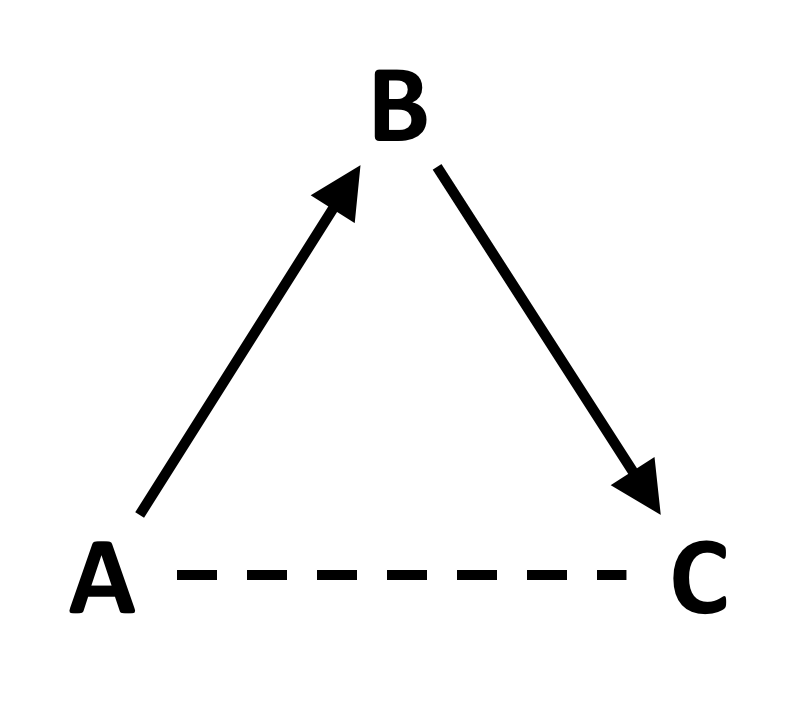
\includegraphics[width=0.7\linewidth]{Images/CDT_brokerage} \end{minipage}  & \begin{minipage}{.2\textwidth} \centering 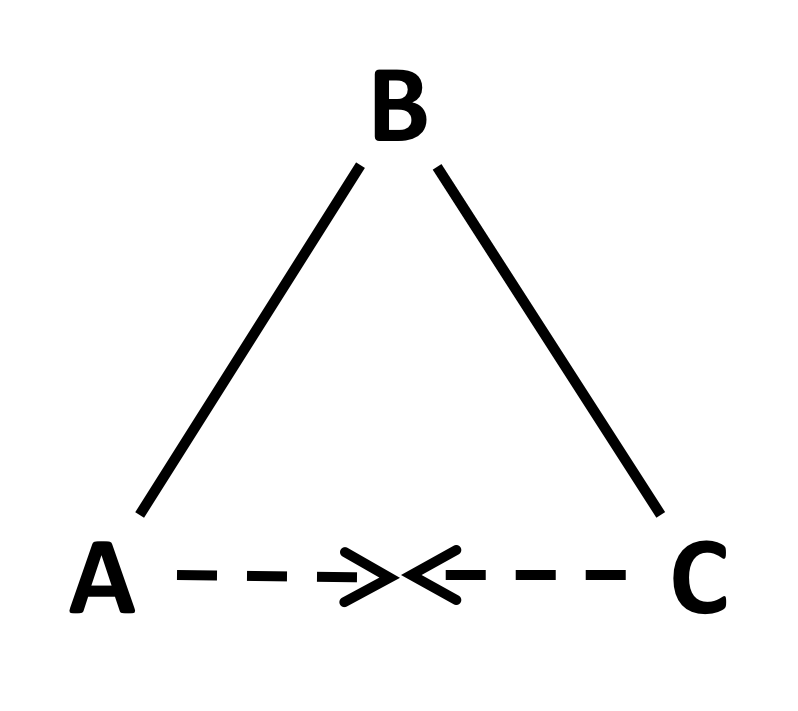
\includegraphics[width=0.7\linewidth]{Images/TG_brokerage_1} \end{minipage}  & \begin{minipage}{.2\textwidth} \centering 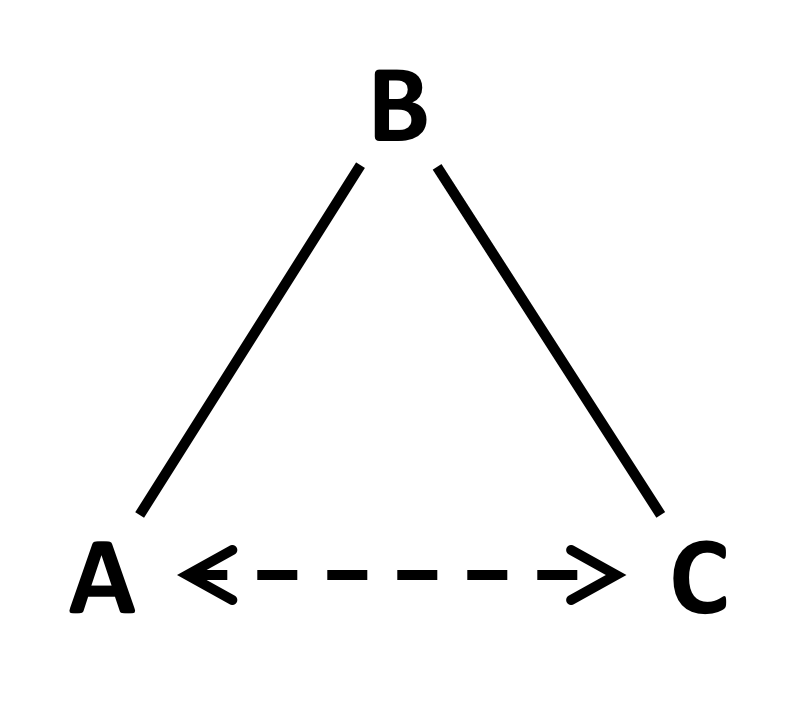
\includegraphics[width=0.7\linewidth]{Images/TI_brokerage} \end{minipage}   \\
	&  &  & \begin{minipage}{.2\textwidth} \centering 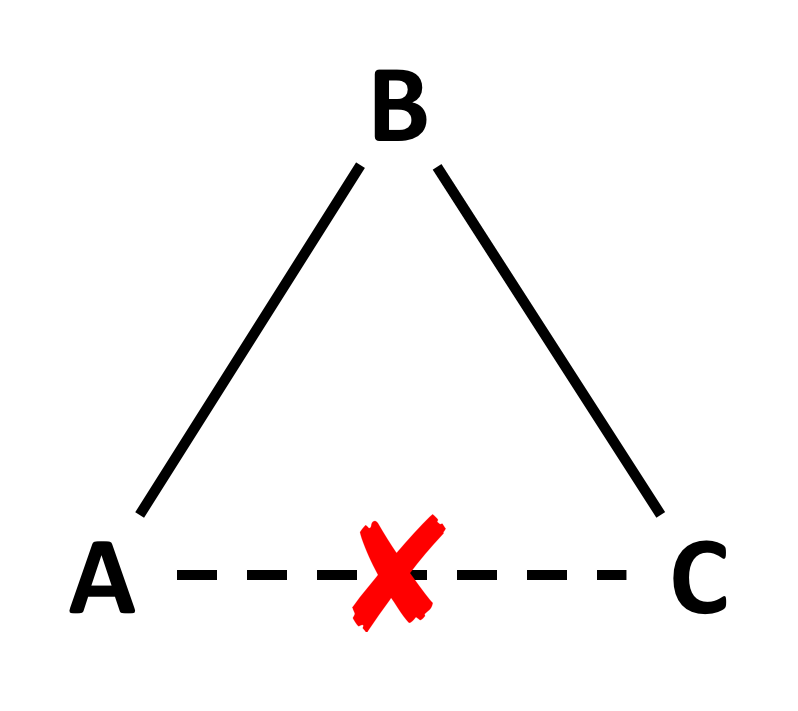
\includegraphics[width=0.7\linewidth]{Images/TG_brokerage_2} \end{minipage}  &  \\
	\midrule
	Open network\\(absence of A-C tie) & B transfers information, knowledge, or other resources between A and C, where A and C have no prospect of meeting. & B plays A and C against one another or keeps A and C apart. & B introduces A and C where A and C have no prior tie. &
	\midrule
	Closed Network\\(presence of A-C tie) & B facilitates transfer between A and C and may help synthesise new knowledge. & B cultivates conflict,competition, or separation between A and C (divide et impera) & B coordinates new collaborative action between A and C. & \\ 
	\bottomrule
\end{tabularx}
\end{table}

With \emph{tertius iungens} brokerage, a third party introduces or facilitates interaction between two other parties. While \emph{tertius gaudens} exploits disconnection or negative ties, \emph{teritius iungens} actively pursues coordination. \emph{Tertius iungens} brokerage is most opportune when the broker detects opportunities to connect complementary, rather than redundant, alter attributes such as resources and abilities \citep{obstfeld2014brokerage}. Both conduit and iungens draw on knowledge articulation, or the social process by which knowledge is made more explicit, useful, or relevant to the situation at hand \citep{obstfeld2005social,obstfeld2011saying,obstfeld2012creative}.

\citet{cohen1990absorptive} see brokers with diverse expertise and contacts playing a key role in the acquisition of knowledge. They believe a diversity of internal perspectives is important to counter resistance towards external knowledge or ideas. From an open innovation perspective, \emph{tertius iungens} brokerage is quite important, especially in the early stages of collaboration, when many actors do not know fellow collaborators in partner organisations. Not only that, knowledge held by third parties is also likely to be unfamiliar. Once ties have been established through \emph{tertius iungens} brokerage, \emph{conduit} brokerage is needed to sustain swift trust and help synthesise and transform knowledge into novel ideas \citep{fleming2007collaborative,lingo2010nexus,quintane2016brokers}. \citet{gould1989structures} describe \emph{conduit} brokerage in terms of \emph{coordination}, \emph{liaison}, \emph{itinerant}, \emph{representative}, and \emph{gatekeeper} roles (Table \ref{gf_params}). Each role expresses a different power dynamic and one should be able to use the relative proportion of each role to characterise power-relations in open innovation collaborations. \medskip

\begin{table}[]
	\small
	\centering
	\caption{Gould-Fernandez brokerage roles. After \citet{gould1989structures} and \citet{butts2016package}.}
	\label{gf_params}
	\begin{tabularx}{\textwidth}{@{}lcl@{}}
		\toprule
		\multicolumn{1}{c}{Role} & \multicolumn{1}{c}{Motif} & \multicolumn{1}{c}{Explanation} \\ \midrule
		Liaison (b\textsubscript{O})			&  \begin{minipage}{.2\textwidth} \centering 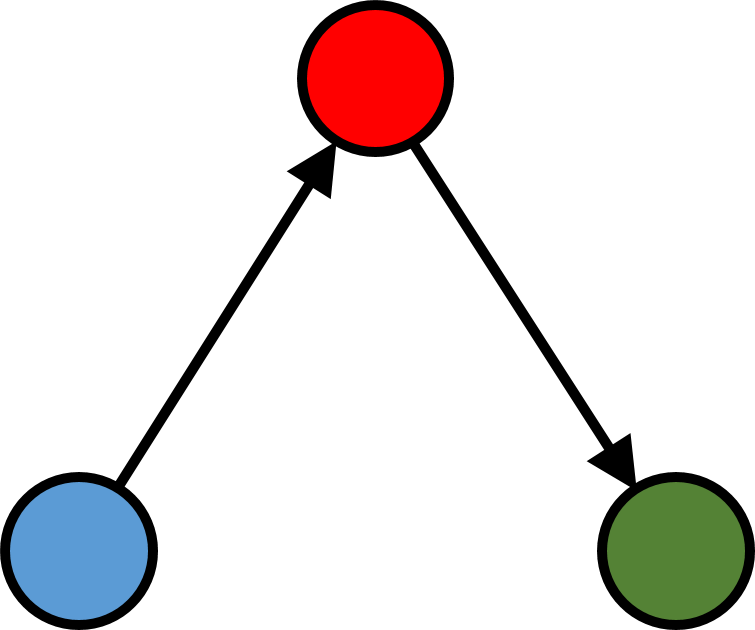
\includegraphics[width=0.4\linewidth]{Images/b_O} \end{minipage}	& \begin{tabular}[c]{l}Broker mediates contact between two\\ individuals from different groups,\\ neither of which is the group to\\ which he or she belongs.\end{tabular}\\ [10ex]
		Representative  (b\textsubscript{IO})	& \begin{minipage}{.2\textwidth} \centering 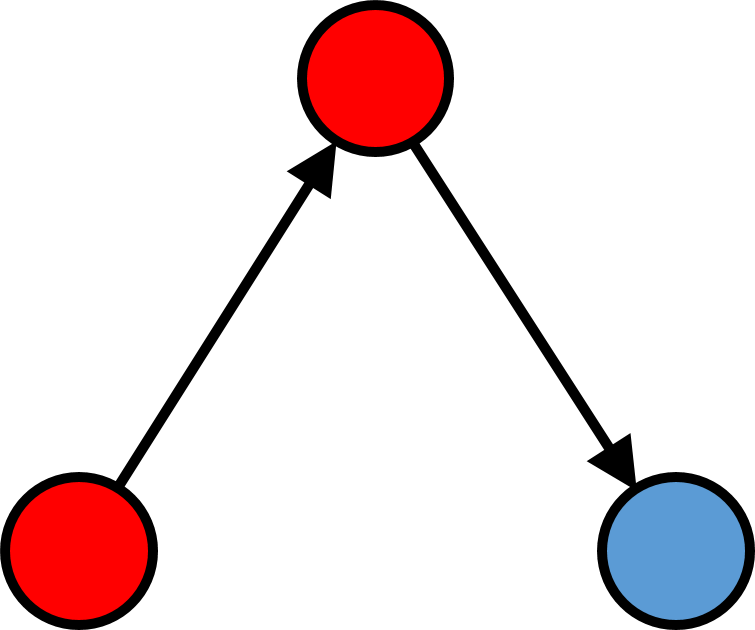
\includegraphics[width=0.4\linewidth]{Images/b_IO} \end{minipage}   & \begin{tabular}[c]{l}Broker mediates an outgoing contact\\ from an in-group member to an\\ out-group member.\end{tabular}\\ [10ex]
		Gatekeeper (b\textsubscript{OI})		& \begin{minipage}{.2\textwidth} \centering 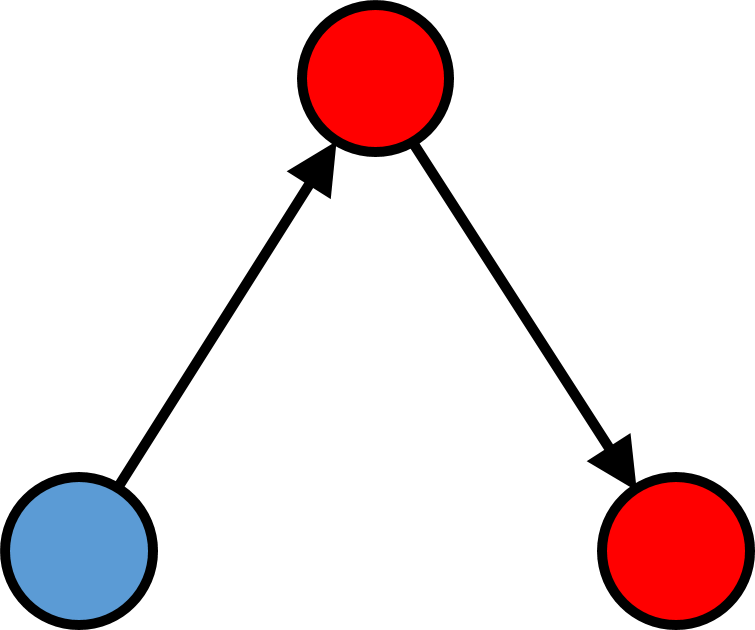
\includegraphics[width=0.4\linewidth]{Images/b_OI} \end{minipage}   & \begin{tabular}[c]{l}Broker mediates an incoming contact\\ from an out-group member to an\\ in-group member. \end{tabular}\\ [10ex]
		Itinerant broker (w\textsubscript{O})	&  \begin{minipage}{.2\textwidth} \centering 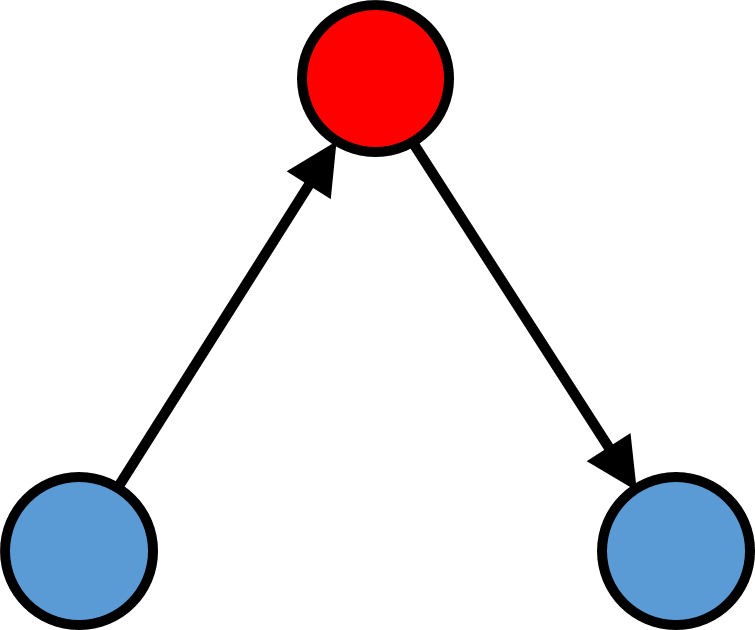
\includegraphics[width=0.4\linewidth]{Images/w_O} \end{minipage}   & \begin{tabular}[c]{l}Broker mediates contact between two\\ individuals from a single group to\\ which he or she does not belong. \end{tabular}\\ [10ex]
		Coordination (w\textsubscript{I})		& \begin{minipage}{.2\textwidth} \centering 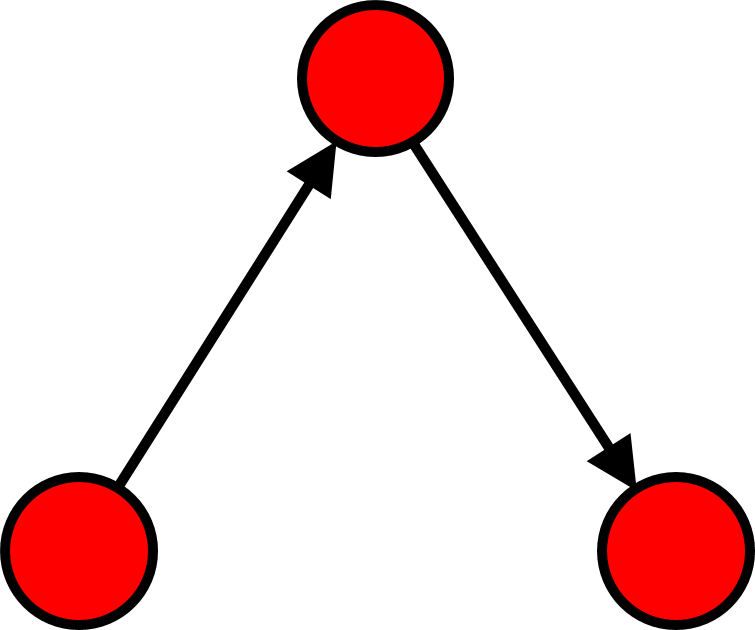
\includegraphics[width=0.4\linewidth]{Images/w_I} \end{minipage}    & \begin{tabular}[c]{l}Broker mediates contact between two\\ individuals from his or her own\\ group. \end{tabular}\\ 
		\bottomrule
	\end{tabularx}
\end{table}

Effective brokerage strategies may require complex combinations and sequences of different brokerage behaviours over time. Skilled brokerage often involves selective deployment of these approaches with different actors or for different objectives. Different combinations of \emph{tertius iungens} and \empg{tertius gaudens} behaviour are necessary to tailor brokerage strategies to match the situation \citep{obstfeld2014brokerage}. 

\citet{tortoriello2010activating} investigate the paradox in which diversity of knowledge and information available across organisational boundaries is necessary to spur innovation, yet at the same time may be a barrier for successful knowledge sharing and integration. Advantages stemming from bridging ties are contingent upon the configuration or microstructure of the ties forming the bridge \citep{tortoriello2010activating,tortoriello2015social}. Common third-party ties facilitate shared understanding, reduce friction due to differences in understanding, and promote cooperation and coordinated actions that are necessary to integrate and take advantage of diverse sources of knowledge \citep{tortoriello2010activating}. Such brokerage is a crucial means by which intra- and inter-organisational networks evolve, expand and drive change \citep{obstfeld2014brokerage}.  \medskip

\section{Summary}

Relative differences in absorptive capacity can impede the flow of knowledge across organisational boundaries, create power imbalances, and undermine alliance performance. Tacit knowledge is key in overcoming relative differences in absorptive capacity in open innovation partnerships. Communicating tacit knowledge requires significant effort and people need to be sufficiently motivated to share or seek out tacit knowledge. Tacit knowledge is a source of power. Because it is a valuable resource accumulated over a lifetime of experience, people are not going to hand over their tacit knowledge just like that. They will be very selective in who they choose to share their tacit knowledge with. People who share their tacit knowledge are empowering others. They are more likely to share their tacit knowledge with others they deem trustworthy. Tacit knowledge is more likely to be shared between actors whose power is not too imbalanced.

% reciprocity
% swift trust
% brokerage

